%%%%%%%%%%%%%%%%%%%%%%%%%%%%%%%%%%%%%%%%%%%%%%%%%%%%%%%%%%%%%%%%%%%%%%%%%
\begin{figure}[p]
 \begin{center}
  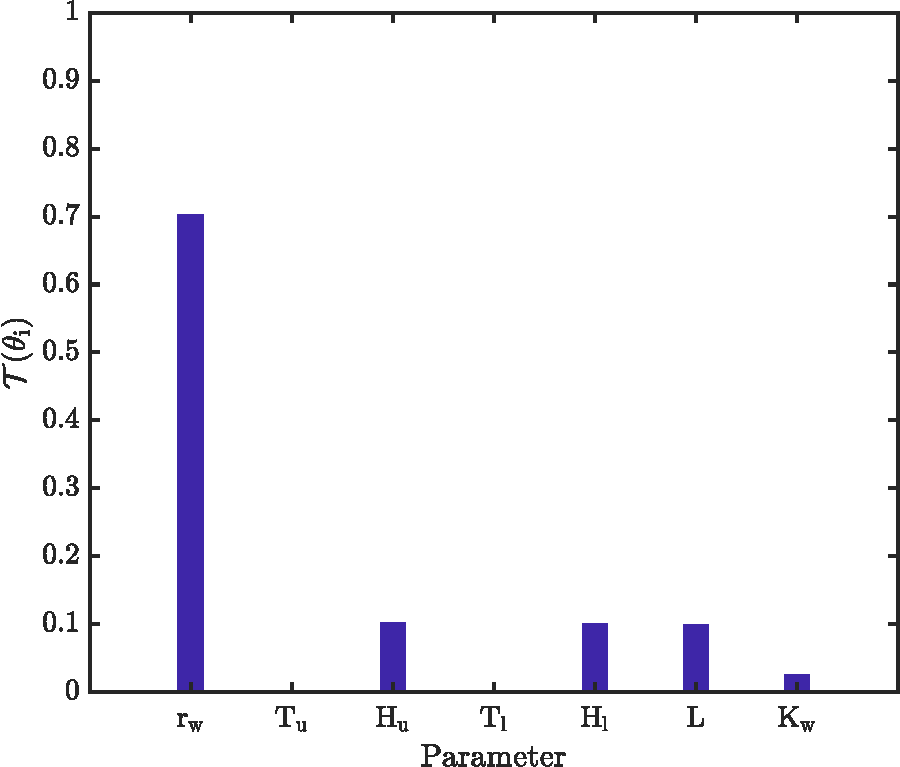
\includegraphics[width=0.70\textwidth]{./Figures/sense_borehole}
\caption{Sobol' total effect sensitivity index for uncertain parameters in the borehole
function (Eq.~\ref{eq:bore}).}
\label{fig:sense_bore}
\end{center}
\end{figure}

\clearpage

%%%%%%%%%%%%%%%%%%%%%%%%%%%%%%%%%%%%%%%%%%%%%%%%%%%%%%%%%%%%%%%%%%%%%%%%%
\begin{figure}[p]
 \begin{center}
  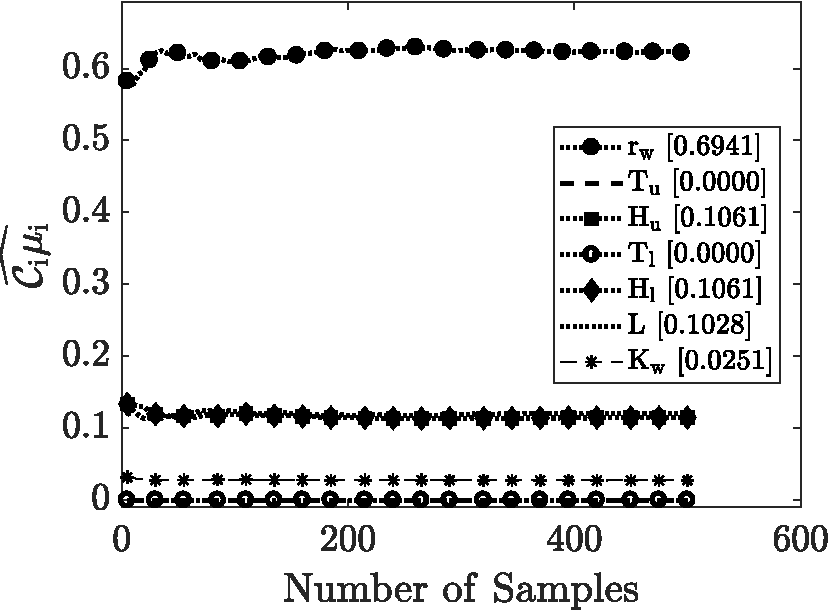
\includegraphics[width=0.70\textwidth]{./Figures/ub_conv_borehole}
\caption{Estimates of the screening parameter ($\hat{\mathcal{C}_i\mu_i}$) is plotted 
against number of samples considered for evaluating $\mu_i$. Corresponding estimates
for the converged Sobol' total effect index ($\mathcal{T}(\theta_i)$) in each case is also included in the
legend.}
\label{fig:screen_bore}
\end{center}
\end{figure}

\clearpage

